\section{Paràmetres de cerca no funcionals}

\subsection{Introducció i demostració}

\paragraph{}
Com ja havíem anunciat en la funcionalitat cerca de persones a l'arbre familiar, exposada en l'apartat~\ref{sec:searchTree}, sembla que els paràmetres de cerca, referents a les localitzacions i dates de naixement, casament i defunció, pels relatius de la per\-sona cercada, no funcionen.

Introduíem aquest fet ja en la funcionalitat, perquè aquest comportament era detectable en l'entorn `sandbox', però volíem comprovar-ho també a producció. Per fer-ho, utilitzarem el següent conjunt de persones de l'arbre familiar:

\begin{itemize}
    \item Principal persona cercada
    \begin{itemize}
        \item Nom: Maria Eliza
        \item Cognom: Williams
        \item Naixement: 20 September 1857 / La Moille, Bureau, Illinois, United States
        \item Defunció: 9 July 1935 / Los Angeles, California, United States
    \end{itemize}
    \item Parella de la persona cercada
    \begin{itemize}
        \item Nom: Albert
        \item Cognom: Porter
        \item Naixement: 1844
        \item Defunció: 1925
    \end{itemize}
    \item Pare de la persona cercada
    \begin{itemize}
        \item Nom: Solomon
        \item Cognom: Williams
        \item Naixement: 1809
        \item Defunció: 1887
    \end{itemize}
    \item Mare de la persona cercada
    \begin{itemize}
        \item Nom: Frances
        \item Cognom: Prime
        \item Naixement: 1828
        \item Defunció: NA
    \end{itemize}
\end{itemize}

Per demostrar el no funcionament d'alguns dels paràmetres, procedirem a rea\-lit\-zar diferents cerques i a observar-ne els resultats.

En primer lloc, si utilitzem els paràmetres \emph{nom} i \emph{cognom}, de la principal persona cercada, el SDK retorna un total de 52 persones (figura~\ref{fig:maria1}).

\begin{figure}[h]
    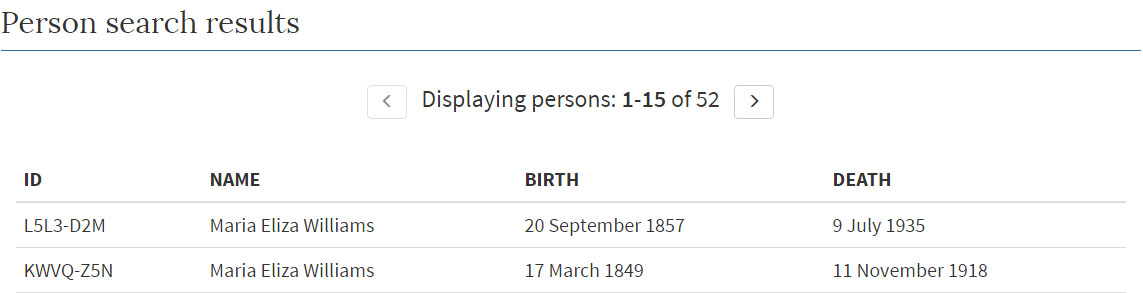
\includegraphics[width=\linewidth]{11.5/01_maria1}
    \centering
    \caption{Cerca amb nom i cognom de la principal persona cercada}\label{fig:maria1}
\end{figure}

En segon lloc, si concretem la informació sobre la principal persona cercada, incloent-hi els paràmetres data i lloc de naixement i data i lloc de defunció, passem a obtenir només la persona que desitgem de l'arbre familiar (figura~\ref{fig:maria2}).

\begin{figure}[h]
    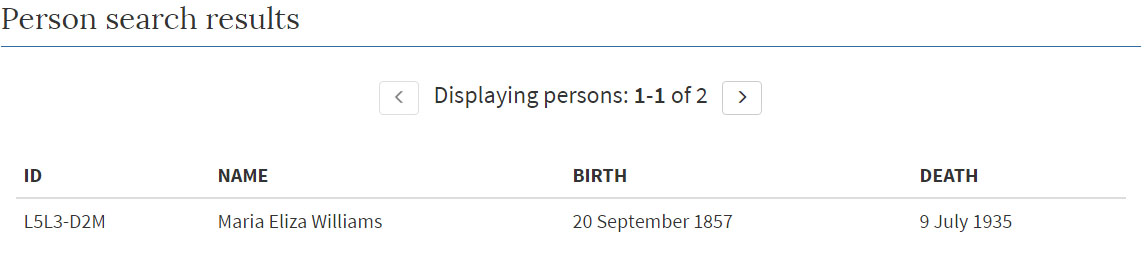
\includegraphics[width=\linewidth]{11.5/02_maria2}
    \centering
    \caption{Cerca detallada o cerca amb nom i cognom dels relatius}\label{fig:maria2}
\end{figure}

De la mateixa forma, per confirmar que la cerca mitjançant els noms i cognoms dels familiars més propers funciona, realitzem una cerca utilitzant només el \emph{nom} i \emph{cognom}, de la principal persona cercada, la parella, el pare i la mare. El resultat, de la mateixa forma que la cerca anterior, només una persona (figura~\ref{fig:maria2}).

Així doncs, es veu clar que els paràmetres \emph{nom} i \emph{cognom} dels relatius, sí que funcionen i és més, ens ajuden a reduir el nombre de resultats, de les 52 persones elegibles utilitzant només el \emph{nom} i \emph{cognom} de la persona cercada, a només 1 resultat.

No obstant això, tan  bon punt afegim qualsevol paràmetre, com per exemple, l'any de naixement del pare, la cerca produeix zero resultats (imatge~\ref{fig:maria3}). El mateix resultat és obtingut, si s'utilitza qualsevol localització o any, relacionat amb els principals esdeveniments, dels relatius més propers de la persona cercada.

\begin{figure}[h]
    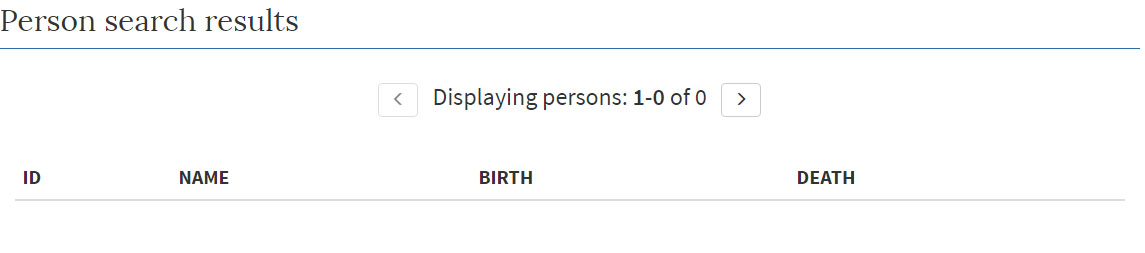
\includegraphics[width=\linewidth]{11.5/03_maria3}
    \centering
    \caption{Cerca amb el paràmetre any de neixement del pare}\label{fig:maria3}
\end{figure}


\subsection{Implicacions del problema}

\paragraph{}
Les implicacions d'aquest problema són bastant evidents. Simplement, aquests paràmetres de cerca no poden ser utilitzats.

Desconeixem el motiu pel qual aquests paràmetres es troben especificats en la documentació oficial com a utilitzables, però la realitat és, que ni la mateixa organit\-zació, els utilitza en la seva funcionalitat de cerca a l'arbre genealògic. (figura~\ref{fig:searchofi}).

\begin{figure}[h]
    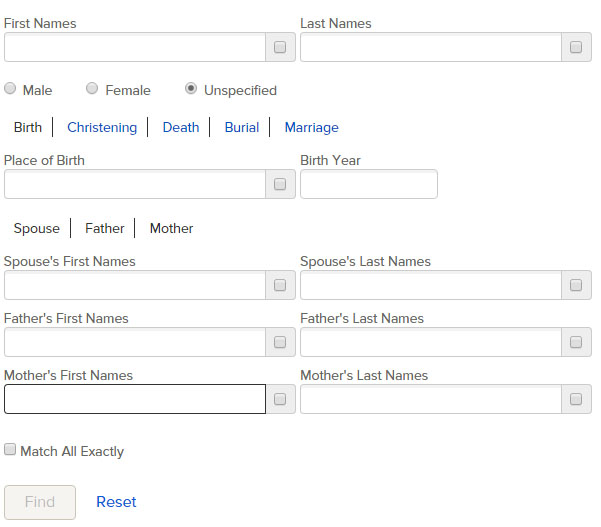
\includegraphics[scale=0.4]{11.5/04_oficialSearcher}
    \centering
    \caption{Formulari oficial de cerca a l'arbre familiar de FamilySearch}\label{fig:searchofi}
\end{figure}
